 Consider $\vec{A},\vec{B},\vec{C}$ are three points of a triangle $\triangle ABC$, $\vec{D}, \vec{B}, \vec{C}$ are three points of another triangle $\triangle DBC$, both triangles having same base BC and $\vec{B}$ at origin, then
\begin{align}
    \label{eq:solutions/1/3/1}
    \vec{A}-\vec{B}=\vec{A}\\
    \label{eq:solutions/1/3/2}
    \vec{C}-\vec{B}=\vec{C}\\
    \label{eq:solutions/1/3/3}
    \vec{D}-\vec{B}=\vec{D}
\end{align}
\renewcommand{\thefigure}{1}
\begin{figure}[!ht]
\centering
\resizebox{\columnwidth}{!}{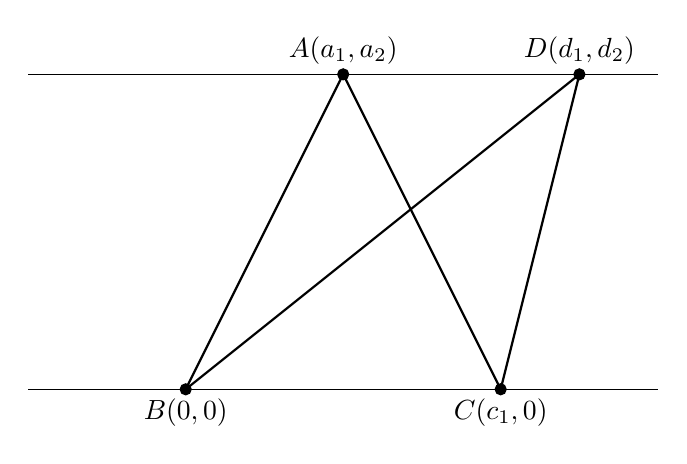
\begin{tikzpicture}
\draw (-2,0) -- (6,0); 
\draw (-2,4) -- (6,4);
\filldraw[black] (0,0) circle (2pt) node[anchor=north] {$B (0,0)$};
\filldraw[black] (2,4) circle (2pt) node[anchor=south] {$A (a_1,a_2)$};
\filldraw[black] (4,0) circle (2pt) node[anchor=north] {$C (c_1,0)$};
\filldraw[black] (5,4) circle (2pt) node[anchor=south] {$D (d_1,d_2)$};
\draw[black,thick] (0,0) -- (2,4);
\draw[black,thick] (4,0) -- (2,4);
\draw[black,thick] (0,0) -- (5,4);
\draw[black,thick] (4,0) -- (5,4);
\draw[black] (4,0) -- (0,0);
\end{tikzpicture}
}
\caption{$\triangle ABC$ and $\triangle DBC$ with BC as common base}
\label{eq:solutions/1/3/fig:1.2}
\end{figure}
The area of the triangle $\triangle ABC$ is,
\begin{align}
    \label{eq:solutions/1/3/4}
    Area\brak{\triangle ABC} = \frac{1}{2}\norm{\brak{\vec{A} - \vec{B}} \times \brak{\vec{C} - \vec{B}}}
\end{align}
Substituting \eqref{eq:solutions/1/3/1} and \eqref{eq:solutions/1/3/2} in \eqref{eq:solutions/1/3/4}, 
\begin{align}
    \label{eq:solutions/1/3/ABC}
    \implies Area\brak{\triangle ABC} = \frac{1}{2}\norm{\brak{\vec{A} \times \vec{C}}}
\end{align}
The area of the triangle $\triangle DBC$ is,
\begin{align}
    \label{eq:solutions/1/3/5}
    Area\brak{\triangle ABC} = \frac{1}{2}\norm{\brak{\vec{D} - \vec{B}} \times \brak{\vec{C} - \vec{B}}}
\end{align}   
Substituting \eqref{eq:solutions/1/3/2} and \eqref{eq:solutions/1/3/3} in \eqref{eq:solutions/1/3/5}, 
\begin{align}
    \label{eq:solutions/1/3/DBC}
    \implies Area\brak{\triangle DBC} = \frac{1}{2}\norm{\brak{\vec{D} \times \vec{C}}}
\end{align}
Given the area of $\triangle ABC$ is equal to the area $\triangle DBC$, from equations \eqref{eq:solutions/1/3/ABC} and \eqref{eq:solutions/1/3/DBC}
\begin{align}
    \label{eq:solutions/1/3/modeq}
    \frac{1}{2}\norm{\brak{\vec{A} \times \vec{C}}} = \frac{1}{2}\norm{\brak{\vec{D} \times \vec{C}}}
\end{align}
Squaring on both sides of the equation \eqref{eq:solutions/1/3/modeq}, we get
\begin{align}
    \norm{\brak{\vec{A} \times \vec{C}}}^2 = \norm{\brak{\vec{D} \times \vec{C}}}^2
\end{align}
\begin{align}
    \implies\brak{\vec{A}\times\vec{C}}^T \brak{\vec{A}\times\vec{C}} = \brak{\vec{D}\times\vec{C}}^T \brak{\vec{D}\times\vec{C}}
\end{align}
\begin{align}
    \implies \brak{\vec{A}^T\vec{A}}\brak{\vec{C}^T\vec{C}} - \brak{\vec{A}^T\vec{C}}\brak{\vec{C}^T\vec{A}} =\\ \brak{\vec{D}^T\vec{D}}\brak{\vec{C}^T\vec{C}} - \brak{\vec{D}^T\vec{C}}\brak{\vec{C}^T\vec{D}}
\end{align}
\begin{align}
    \label{eq:solutions/1/3/eq11}
    \implies\norm{\vec{A}}^2\norm{\vec{C}}^2 - \brak{\vec{A}^T\vec{C}}^2 = \norm{\vec{D}}^2\norm{\vec{C}^2} - \brak{\vec{D}^T\vec{C}}^2 
\end{align}
Let $\vec{A}=\myvec{a1\\a2}$, $\vec{C}=\myvec{c_1\\0}$ and $\vec{D}=\myvec{d_1\\d_2}$ .Then equation \eqref{eq:solutions/1/3/eq11} can be written as,
\begin{align}
    \label{eq:solutions/1/3/lbo}
    \brak{a_1^2+a_2^2}\brak{c_1^2}-\brak{a_1c_1}^2 = \brak{d_1^2+d_2^2}\brak{c_1^2} - \brak{d_1c_1}^2
\end{align}
\begin{align}
    \implies a_2 = d_2
\end{align}
Now we have,
\begin{align}
    \label{eq:solutions/1/3/eq14}
    \brak{\vec{D}-\vec{A}}=\myvec{d_1-a_1\\d_2-a_2} = \myvec{d_1-a_1\\0}\\ 
    \label{eq:solutions/1/3/eq15}
    \brak{\vec{C}-\vec{B}} = \myvec{c_1-0 \\ 0-0} = \myvec{c_1 \\ 0}
\end{align}
From equations \eqref{eq:solutions/1/3/eq14} and \eqref{eq:solutions/1/3/eq15}, we can say
\begin{align}
    \brak{\vec{D}-\vec{A}}=\frac{d_1-a_1}{c_1}\brak{\vec{C}-\vec{B}}\\
    \label{eq:solutions/1/3/lst}
    \implies \brak{\vec{D}-\vec{A}}=k\brak{\vec{C}-\vec{B}}
\end{align}
where $k$ is a constant. From the equation \eqref{eq:solutions/1/3/lst}, we can say that $AD \parallel BC$. Hence the two triangles $\triangle ABC$ and $\triangle DBC$ lie between the same parallels AD and BC
